\documentclass[notes,11pt, aspectratio=169]{beamer}

\usepackage{pgfpages}
\setbeameroption{hide notes} % Only slide

\usepackage{array}
\usepackage{tikz}
\usepackage{verbatim}
\setbeamertemplate{note page}{\pagecolor{gray!5}\insertnote}
\usetikzlibrary{positioning}
\usetikzlibrary{snakes}
\usetikzlibrary{calc}
\usetikzlibrary{arrows}
\usetikzlibrary{decorations.markings}
\usetikzlibrary{shapes.misc}
\usetikzlibrary{matrix,shapes,arrows,fit,tikzmark}
\usepackage{amsmath}
\usepackage{mathpazo}
\usepackage{hyperref}
\usepackage{lipsum}
\usepackage{multimedia}
\usepackage{graphicx}
\usepackage{multirow}
\usepackage{dcolumn}
\usepackage{bbm}
\newcolumntype{d}[0]{D{.}{.}{5}}

\usepackage{changepage}
\usepackage{appendixnumberbeamer}

\usepackage[space]{grffile}
\usepackage{booktabs}

% Colors
\definecolor{blue}{RGB}{0,114,178}
\definecolor{red}{RGB}{213,94,0}
\definecolor{yellow}{RGB}{240,228,66}
\definecolor{green}{RGB}{0,158,115}
\definecolor{solutionbg}{RGB}{240,248,240}
\definecolor{solutionframe}{RGB}{0,158,115}

% Solution box environment for worked answers
\usepackage{tcolorbox}
\newtcolorbox{solutionbox}[1][]{
  enhanced,
  colback=solutionbg,
  colframe=solutionframe,
  boxrule=0pt,
  leftrule=3pt,
  arc=0pt,
  left=8pt,
  right=8pt,
  top=6pt,
  bottom=6pt,
  fonttitle=\bfseries,
  title={#1},
  attach boxed title to top left={yshift=-2mm, xshift=5mm},
  boxed title style={colback=solutionframe, colframe=solutionframe, size=small, arc=2pt}
}

\hypersetup{
  colorlinks=false,
  linkbordercolor = {white},
  linkcolor = {blue}
}

\definecolor{MyBackground}{RGB}{255,253,218}

\newenvironment{transitionframe}{
  \setbeamercolor{background canvas}{bg=white}
  \begin{frame}}{
    \end{frame}
}

\setbeamercolor{frametitle}{fg=blue}
\setbeamercolor{title}{fg=black}
\setbeamertemplate{footline}[frame number]
\setbeamertemplate{navigation symbols}{}
\setbeamertemplate{itemize items}{-}
\setbeamercolor{itemize item}{fg=blue}
\setbeamercolor{itemize subitem}{fg=blue}
\setbeamercolor{enumerate item}{fg=blue}
\setbeamercolor{enumerate subitem}{fg=blue}
\setbeamercolor{button}{bg=MyBackground,fg=blue,}

\setbeamercolor{section in toc}{fg=blue}
\setbeamercolor{subsection in toc}{fg=red}
\setbeamersize{text margin left=1em,text margin right=1em}

\newenvironment{wideitemize}{\itemize\addtolength{\itemsep}{10pt}}{\enditemize}
\newenvironment{wideenumerate}{\enumerate\addtolength{\itemsep}{10pt}}{\endenumerate}

\title[]{\textcolor{blue}{ECN 594: Vertical Relationships}}
\author[PGP]{}
\institute[FRBNY]{\small{\begin{tabular}{c c c}
Nicholas Vreugdenhil \\
\end{tabular}}}
\date{\today}

\begin{document}

% Title Slide
\begin{frame}
\maketitle
  \centering
\end{frame}

\begin{frame}{Plan}
  \begin{wideenumerate}
    \item \textbf{Vertical relationships: upstream and downstream}
    \item Double marginalization problem
    \item Solutions: integration and two-part tariffs
    \item Vertical restraints
    \item The free-rider problem
    \item Antitrust implications
  \end{wideenumerate}
\end{frame}

%%%%%%%%%%%%%%%%%%%%%%%%%%%%%%%%%%%%%%%%%%%%%%%%%%%%%%%%%%%%%
% DOUBLE MARGINALIZATION
%%%%%%%%%%%%%%%%%%%%%%%%%%%%%%%%%%%%%%%%%%%%%%%%%%%%%%%%%%%%%

\begin{frame}{Vertical relationships}
	\begin{wideitemize}
		\item \textbf{Vertical structure:} Production chain from raw materials to consumers
		\item \textbf{Upstream:} Manufacturers, wholesalers
		\item \textbf{Downstream:} Retailers, distributors
		\item \textbf{Examples:}
		\begin{wideitemize}
			\vspace{5pt}
			\item Car manufacturer $\rightarrow$ dealer
			\item Beverage company $\rightarrow$ restaurant
			\item Book publisher $\rightarrow$ bookstore
		\end{wideitemize}
		\item Key question: How should these relationships be structured?
	\end{wideitemize}
\end{frame}

\begin{frame}{Plan}
  \begin{wideenumerate}
    \item Vertical relationships: upstream and downstream
    \item \textbf{Double marginalization problem}
    \item Solutions: integration and two-part tariffs
    \item Vertical restraints
    \item The free-rider problem
    \item Antitrust implications
  \end{wideenumerate}
\end{frame}

\begin{frame}{Double marginalization: setup}
	\begin{wideitemize}
		\item \textbf{Upstream monopolist} (manufacturer): produces at $MC = c$
		\item Sells to \textbf{downstream monopolist} (retailer) at price $w$
		\item Retailer sells to consumers at price $p$
		\item Consumer demand: $q = D(p)$
		\item \textbf{Problem:} Each firm adds its own markup
	\end{wideitemize}
\end{frame}

\begin{frame}{Double marginalization: the chain}
	\begin{center}
		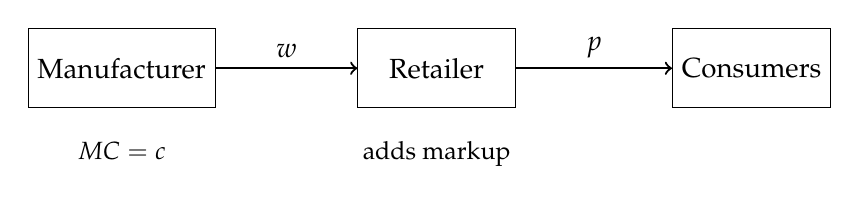
\begin{tikzpicture}[node distance=2.5cm, auto]
			\node[draw, rectangle, minimum width=2cm, minimum height=1cm] (M) {Manufacturer};
			\node[draw, rectangle, minimum width=2cm, minimum height=1cm, right of=M, node distance=4cm] (R) {Retailer};
			\node[draw, rectangle, minimum width=2cm, minimum height=1cm, right of=R, node distance=4cm] (C) {Consumers};

			\draw[->, thick] (M) -- node[above] {$w$} (R);
			\draw[->, thick] (R) -- node[above] {$p$} (C);

			\node[below=0.3cm of M] {\small $MC = c$};
			\node[below=0.3cm of R] {\small adds markup};
		\end{tikzpicture}
	\end{center}
	\vspace{10pt}
	\begin{wideitemize}
		\item Manufacturer: sets $w > c$ (first markup)
		\item Retailer: sets $p > w$ (second markup)
		\item Result: $p$ is ``too high'' relative to integrated monopolist
	\end{wideitemize}
\end{frame}

\begin{frame}{Double marginalization: intuition}
	\begin{wideitemize}
		\item Each firm ignores the effect of its markup on the other
		\item Manufacturer doesn't fully account for:
		\begin{wideitemize}
			\vspace{5pt}
			\item Higher $w$ $\rightarrow$ higher $p$ $\rightarrow$ lower $q$ $\rightarrow$ lower profits for both
		\end{wideitemize}
		\item This is a \textbf{vertical externality}
		\item Integrated monopolist would set lower price!
		\item \textbf{Paradox:} More competition (vertical separation) $\rightarrow$ higher price
	\end{wideitemize}
\end{frame}

\begin{frame}{Worked example: Double marginalization}
	\begin{wideitemize}
		\item Consumer demand: $q = 100 - p$
		\item Manufacturer: $MC = 20$
		\item Retailer: no additional costs (just buys from manufacturer at $w$)
		\item \textbf{Questions:}
		\item (a) Find the price and profit of an integrated monopolist
		\item (b) Find the prices and profits with separate firms
		\item (c) Compare total industry profits
	\end{wideitemize}
	\vspace{10pt}
	\centering
	\textit{Take 7 minutes.}
\end{frame}

\begin{frame}{Worked example: Integration (solution a)}
	\begin{solutionbox}[Solution]
		\begin{wideitemize}
			\item \textbf{Integrated monopolist:}
			\item Inverse demand: $p = 100 - q$
			\item $MR = 100 - 2q$
			\item Set $MR = MC$: $100 - 2q = 20 \Rightarrow q = 40$
			\item $p = 100 - 40 = 60$
			\item $\pi^{Int} = (60 - 20) \times 40 = 1600$
		\end{wideitemize}
	\end{solutionbox}
\end{frame}

\begin{frame}{Worked example: Separation (solution b)}
	\begin{solutionbox}[Solution]
		\begin{wideitemize}
			\item \textbf{Step 1: Retailer's problem} (given $w$)
			\item Retailer's cost is $w$, faces demand $q = 100 - p$
			\item $MR_R = 100 - 2q$, $MC_R = w$
			\item Set $MR_R = MC_R$: $100 - 2q = w \Rightarrow q = (100 - w)/2$
			\item $p = 100 - q = (100 + w)/2$
			\item Retailer profit: $\pi_R = (p - w)q = \left(\frac{100 - w}{2}\right)^2$
		\end{wideitemize}
	\end{solutionbox}
\end{frame}

\begin{frame}{Worked example: Separation (solution b, cont.)}
	\begin{solutionbox}[Solution]
		\begin{wideitemize}
			\item \textbf{Step 2: Manufacturer's problem}
			\item Anticipates retailer's response: $q = (100 - w)/2$
			\item Manufacturer profit: $\pi_M = (w - 20) \times \frac{100 - w}{2}$
			\item FOC: $\frac{\partial \pi_M}{\partial w} = \frac{100 - w}{2} - \frac{w - 20}{2} = 0$
			\item $100 - w = w - 20 \Rightarrow w = 60$
			\item Then: $q = (100 - 60)/2 = 20$, $p = (100 + 60)/2 = 80$
			\item $\pi_M = (60 - 20) \times 20 = 800$
			\item $\pi_R = (80 - 60) \times 20 = 400$
		\end{wideitemize}
	\end{solutionbox}
\end{frame}

\begin{frame}{Worked example: Comparison (solution c)}
	\begin{solutionbox}[Solution]
		\begin{center}
			\begin{tabular}{|l|c|c|}
				\hline
				& \textbf{Integrated} & \textbf{Separated} \\
				\hline
				Final price & 60 & 80 \\
				Quantity & 40 & 20 \\
				Total profit & 1600 & 1200 \\
				\hline
			\end{tabular}
		\end{center}
		\vspace{10pt}
		\begin{wideitemize}
			\item Separation: price 33\% higher, quantity 50\% lower
			\item Industry profits 25\% lower with separation
			\item Consumers also worse off (higher $p$, lower $q$)
			\item \textbf{Everyone loses} from double marginalization!
		\end{wideitemize}
	\end{solutionbox}
\end{frame}

\begin{frame}{Plan}
  \begin{wideenumerate}
    \item Vertical relationships: upstream and downstream
    \item Double marginalization problem
    \item \textbf{Solutions: integration and two-part tariffs}
    \item Vertical restraints
    \item The free-rider problem
    \item Antitrust implications
  \end{wideenumerate}
\end{frame}

\begin{frame}{Solutions to double marginalization}
	\begin{wideenumerate}
		\item \textbf{Vertical integration}
		\begin{wideitemize}
			\vspace{3pt}
			\item Manufacturer buys retailer (or vice versa)
			\item Eliminates double markup
		\end{wideitemize}
		\item \textbf{Two-part tariff}
		\begin{wideitemize}
			\vspace{3pt}
			\item Set $w = MC$ (no wholesale markup)
			\item Charge franchise fee $F$ to extract retailer profits
		\end{wideitemize}
		\item \textbf{Resale price maintenance (RPM)}
		\begin{wideitemize}
			\vspace{3pt}
			\item Manufacturer sets final price directly
			\item Controversial under antitrust law
		\end{wideitemize}
	\end{wideenumerate}
\end{frame}

\begin{frame}{Two-part tariff solution}
	\begin{wideitemize}
		\item Manufacturer charges:
		\begin{wideitemize}
			\vspace{5pt}
			\item Wholesale price: $w = c = MC$ (at cost)
			\item Franchise fee: $F$
		\end{wideitemize}
		\item With $w = MC$, retailer sets integrated monopoly price
		\item Retailer earns $\pi^{Int}$ minus $F$
		\item Manufacturer sets $F = \pi^{Int}$ to extract all profit
		\item \textbf{Result:}
		\begin{wideitemize}
			\vspace{5pt}
			\item Price = integrated monopoly price
			\item Total profit = integrated monopoly profit
			\item Captured by manufacturer through $F$
		\end{wideitemize}
	\end{wideitemize}
\end{frame}

\begin{frame}{Practice: Double marginalization}
	\begin{wideitemize}
		\item \textbf{Question:} Consumer demand is $q = 200 - 2p$.
		\item Manufacturer: $MC = 30$, sells at $w$ to retailer.
		\item Retailer: no additional costs, sells at $p$ to consumers.
		\item (a) What is the integrated monopoly price and profit?
		\item (b) What is the final price with vertical separation?
	\end{wideitemize}
	\vspace{10pt}
	\centering
	\textit{Take 5 minutes.}
\end{frame}

\begin{frame}{Practice: Double marginalization (solution)}
	\begin{solutionbox}[Solution]
		\begin{wideitemize}
			\item Inverse demand: $p = 100 - q/2$
			\item \textbf{(a) Integrated:} $MR = 100 - q$, set $MR = MC$:
			\begin{align*}
				100 - q = 30 \Rightarrow q = 70, \quad p = 65
			\end{align*}
			\item $\pi^{Int} = (65-30) \times 70 = 2450$
			\item \textbf{(b) Separation:} Retailer: $q = (100-w) = 100-w$
			\item Actually: $q = 100 - w$ and $p = (100+w)/2$
			\item Manufacturer: $\max_w (w-30)(100-w)/2$
			\item FOC: $w = 65$, then $q = 35$, $p = 82.5$
		\end{wideitemize}
	\end{solutionbox}
\end{frame}

\begin{frame}{When double marginalization doesn't apply}
	\begin{wideitemize}
		\item \textbf{Competitive retail:} Many retailers $\Rightarrow$ no downstream markup
		\item \textbf{Bargaining power:} Retailer negotiates for $w = MC$
		\item \textbf{Vertical contracts:} Two-part tariffs, RPM
		\item \textbf{Common ownership:} Integrated firms
		\item \textbf{Key insight:} Double marginalization requires:
		\begin{wideenumerate}
			\vspace{5pt}
			\item Market power at both levels
			\item Linear pricing ($w$ per unit only)
		\end{wideenumerate}
	\end{wideitemize}
\end{frame}

\begin{frame}{Practice: T/F on double marginalization}
	\begin{wideitemize}
		\item \textbf{True, False, or NEI:}
		\item (a) Double marginalization makes consumers worse off.
		\item (b) If the retailer is a perfect competitor, double marginalization doesn't occur.
		\item (c) Vertical integration always benefits consumers.
	\end{wideitemize}
	\vspace{10pt}
	\centering
	\textit{Take 2 minutes.}
\end{frame}

\begin{frame}{Practice: T/F on double marginalization (solution)}
	\begin{solutionbox}[Solutions]
		\begin{wideitemize}
			\item \textbf{(a) TRUE.} Higher price, lower quantity. Consumers strictly worse off relative to integrated monopoly.
			\item \textbf{(b) TRUE.} Competitive retailers have zero markup ($p = w$). Only manufacturer's markup remains, so no ``double'' margin.
			\item \textbf{(c) FALSE.} Integration helps consumers IF it replaces separation. But if manufacturer was already using two-part tariff, integration may not change anything.
		\end{wideitemize}
	\end{solutionbox}
\end{frame}

\begin{frame}{Real-world examples: Vertical relationships}
	\begin{wideitemize}
		\item \textbf{Auto industry:}
		\begin{wideitemize}
			\vspace{3pt}
			\item Manufacturers $\rightarrow$ dealers
			\item Dealers have territorial exclusivity
		\end{wideitemize}
		\item \textbf{Beer industry:}
		\begin{wideitemize}
			\vspace{3pt}
			\item Breweries $\rightarrow$ distributors $\rightarrow$ retailers
			\item Three-tier system mandated in many US states
		\end{wideitemize}
		\item \textbf{Tech platforms:}
		\begin{wideitemize}
			\vspace{3pt}
			\item App stores take 30\% commission
			\item This is a form of wholesale markup
		\end{wideitemize}
	\end{wideitemize}
\end{frame}

\begin{frame}{Successive oligopoly}
	\begin{wideitemize}
		\item What if there are multiple firms at each level?
		\item \textbf{Upstream oligopoly $\rightarrow$ Downstream oligopoly}
		\item Results depend on:
		\begin{wideitemize}
			\vspace{5pt}
			\item Number of firms at each level
			\item Type of competition (Cournot vs Bertrand)
			\item Bargaining power
		\end{wideitemize}
		\item General result: more competition at either level reduces final price
		\item But double marginalization can still be present
	\end{wideitemize}
\end{frame}

%%%%%%%%%%%%%%%%%%%%%%%%%%%%%%%%%%%%%%%%%%%%%%%%%%%%%%%%%%%%%
% VERTICAL RESTRAINTS
%%%%%%%%%%%%%%%%%%%%%%%%%%%%%%%%%%%%%%%%%%%%%%%%%%%%%%%%%%%%%

\begin{frame}{Plan}
  \begin{wideenumerate}
    \item Vertical relationships: upstream and downstream
    \item Double marginalization problem
    \item Solutions: integration and two-part tariffs
    \item \textbf{Vertical restraints}
    \item The free-rider problem
    \item Antitrust implications
  \end{wideenumerate}
\end{frame}

\begin{frame}{Vertical restraints: overview}
	\begin{wideitemize}
		\item \textbf{Vertical restraints:} Contractual restrictions between upstream/downstream firms
		\item \textbf{Types:}
		\begin{wideenumerate}
			\vspace{5pt}
			\item \textbf{Exclusive dealing:} Retailer can only sell manufacturer's products
			\item \textbf{Exclusive territories:} Retailer has geographic monopoly
			\item \textbf{Resale price maintenance (RPM):} Manufacturer sets retail price
			\item \textbf{Tying:} Must buy product B to get product A
		\end{wideenumerate}
	\end{wideitemize}
\end{frame}

\begin{frame}{Plan}
  \begin{wideenumerate}
    \item Vertical relationships: upstream and downstream
    \item Double marginalization problem
    \item Solutions: integration and two-part tariffs
    \item Vertical restraints
    \item \textbf{The free-rider problem}
    \item Antitrust implications
  \end{wideenumerate}
\end{frame}

\begin{frame}{The free-rider problem}
	\begin{wideitemize}
		\item \textbf{Setup:} Retailer provides services (advice, showroom, etc.)
		\item \textbf{Problem:}
		\begin{wideitemize}
			\vspace{5pt}
			\item Consumer gets service at Retailer A
			\item Buys from Retailer B (lower price, no service)
			\item Retailer A's service investment wasted
		\end{wideitemize}
		\item \textbf{Result:} Retailers under-invest in services
		\item \textbf{Examples:}
		\begin{wideitemize}
			\vspace{5pt}
			\item Electronics stores vs online retailers
			\item Car dealerships and test drives
		\end{wideitemize}
	\end{wideitemize}
\end{frame}

\begin{frame}{Free-rider problem: graphical}
	\begin{center}
		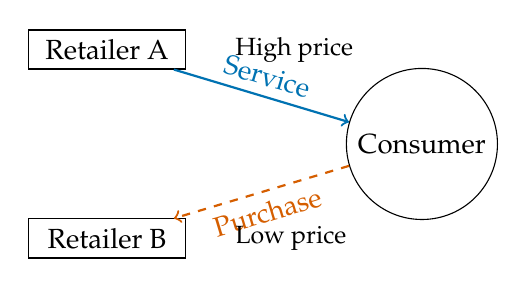
\begin{tikzpicture}[scale=0.8]
			\node[draw, rectangle, minimum width=2cm] (A) at (0,2) {Retailer A};
			\node[draw, rectangle, minimum width=2cm] (B) at (0,-1) {Retailer B};
			\node[draw, circle] (C) at (5,0.5) {Consumer};

			\draw[->, thick, blue] (A) -- node[above, sloped] {Service} (C);
			\draw[->, thick, red, dashed] (C) -- node[below, sloped] {Purchase} (B);

			\node[right=0.5cm of A] {\small High price};
			\node[right=0.5cm of B] {\small Low price};
		\end{tikzpicture}
	\end{center}
	\begin{wideitemize}
		\item Consumer gets service from A but buys from B
		\item A's investment is not rewarded $\Rightarrow$ stops providing service
	\end{wideitemize}
\end{frame}

\begin{frame}{Exclusive dealing}
	\begin{wideitemize}
		\item \textbf{Definition:} Retailer agrees to sell only one manufacturer's products
		\item \textbf{Pro-competitive:}
		\begin{wideitemize}
			\vspace{5pt}
			\item Encourages retailer investment in manufacturer's brand
			\item Prevents free-riding on promotional efforts
		\end{wideitemize}
		\item \textbf{Anti-competitive:}
		\begin{wideitemize}
			\vspace{5pt}
			\item May foreclose rivals from distribution
			\item Especially concerning if many retailers are tied up
		\end{wideitemize}
		\item \textbf{Example:} Beverage exclusivity (Coke vs Pepsi at restaurants)
	\end{wideitemize}
\end{frame}

\begin{frame}{RPM: A closer look}
	\begin{wideitemize}
		\item \textbf{Minimum RPM:} Floor on retail price
		\begin{wideitemize}
			\vspace{5pt}
			\item Prevents discounting
			\item Protects service margins
		\end{wideitemize}
		\item \textbf{Maximum RPM:} Ceiling on retail price
		\begin{wideitemize}
			\vspace{5pt}
			\item Prevents double marginalization!
			\item Generally more benign
		\end{wideitemize}
		\item \textbf{Case law evolution:}
		\begin{wideitemize}
			\vspace{5pt}
			\item Minimum RPM: per se illegal (1911-2007), now rule of reason
			\item Maximum RPM: always rule of reason
		\end{wideitemize}
	\end{wideitemize}
\end{frame}

\begin{frame}{Solutions to free-riding}
	\begin{wideitemize}
		\item \textbf{Resale price maintenance (RPM):}
		\begin{wideitemize}
			\vspace{5pt}
			\item Set minimum retail price
			\item Prevents price competition, preserves margin for services
		\end{wideitemize}
		\item \textbf{Exclusive territories:}
		\begin{wideitemize}
			\vspace{5pt}
			\item Each retailer is local monopolist
			\item No other retailer to free-ride on
		\end{wideitemize}
		\item Both reduce \textbf{intra-brand} competition (same brand, different retailers)
	\end{wideitemize}
\end{frame}

\begin{frame}{Intra-brand vs inter-brand competition}
	\begin{wideitemize}
		\item \textbf{Intra-brand:} Competition among retailers selling same brand
		\begin{wideitemize}
			\vspace{5pt}
			\item Different Toyota dealers competing on price
		\end{wideitemize}
		\item \textbf{Inter-brand:} Competition between different brands
		\begin{wideitemize}
			\vspace{5pt}
			\item Toyota vs Honda
		\end{wideitemize}
		\item \textbf{Vertical restraints often reduce intra-brand competition}
		\item \textbf{Key question for antitrust:}
		\begin{wideitemize}
			\vspace{5pt}
			\item If inter-brand competition is strong, less concern
			\item If inter-brand is weak, restraints may harm consumers
		\end{wideitemize}
	\end{wideitemize}
\end{frame}

\begin{frame}{Practice: Identify the restraint}
	\begin{wideitemize}
		\item \textbf{Which restraint is being used?}
		\item (a) Nike requires retailers to charge at least \$150 for certain shoes.
		\item (b) McDonald's franchises can only sell McDonald's food.
		\item (c) A Pepsi distributor is the only one allowed in a region.
		\item (d) A printer company requires customers to buy its toner.
	\end{wideitemize}
	\vspace{10pt}
	\centering
	\textit{Take 1 minute.}
\end{frame}

\begin{frame}{Plan}
  \begin{wideenumerate}
    \item Vertical relationships: upstream and downstream
    \item Double marginalization problem
    \item Solutions: integration and two-part tariffs
    \item Vertical restraints
    \item The free-rider problem
    \item \textbf{Antitrust implications}
  \end{wideenumerate}
\end{frame}

\begin{frame}{Antitrust analysis of vertical restraints}
	\begin{wideitemize}
		\item \textbf{Rule of reason:} Case-by-case analysis
		\begin{wideitemize}
			\vspace{5pt}
			\item Weigh pro-competitive vs anti-competitive effects
		\end{wideitemize}
		\item \textbf{Pro-competitive justifications:}
		\begin{wideitemize}
			\vspace{5pt}
			\item Solve free-rider problem
			\item Encourage retailer investments
			\item Improve product quality/service
		\end{wideitemize}
		\item \textbf{Anti-competitive concerns:}
		\begin{wideitemize}
			\vspace{5pt}
			\item Facilitate collusion
			\item Exclude competitors
			\item Raise prices without efficiency benefit
		\end{wideitemize}
	\end{wideitemize}
\end{frame}

\begin{frame}{Legal status of vertical restraints}
	\begin{center}
		\begin{tabular}{|l|c|}
			\hline
			\textbf{Restraint} & \textbf{US Legal Status} \\
			\hline
			Maximum RPM & Rule of reason \\
			Minimum RPM & Rule of reason (since 2007) \\
			Exclusive dealing & Rule of reason \\
			Exclusive territories & Rule of reason \\
			Tying & Quasi-per se illegal \\
			\hline
		\end{tabular}
	\end{center}
	\vspace{10pt}
	\begin{wideitemize}
		\item Most restraints evaluated under rule of reason
		\item Need to show harm to competition (not just competitors)
	\end{wideitemize}
\end{frame}

\begin{frame}{Practice: Vertical restraints}
	\begin{wideitemize}
		\item \textbf{True, False, or NEI:}
		\item (a) Exclusive dealing is always anti-competitive.
		\item (b) Maximum RPM can solve double marginalization.
		\item (c) RPM would be unnecessary if retailers didn't compete on price.
	\end{wideitemize}
	\vspace{10pt}
	\centering
	\textit{Take 2 minutes.}
\end{frame}

\begin{frame}{Practice: Vertical restraints (solution)}
	\begin{solutionbox}[Solutions]
		\begin{wideitemize}
			\item \textbf{(a) FALSE.} Exclusive dealing can solve free-rider problems and encourage retailer investment. It's anti-competitive only if it forecloses significant distribution.
			\item \textbf{(b) TRUE.} By setting a maximum retail price, manufacturer can prevent excessive downstream markup.
			\item \textbf{(c) TRUE (essentially).} If retailers don't compete on price (e.g., exclusive territories), there's no free-riding on price. RPM addresses price-based free-riding.
		\end{wideitemize}
	\end{solutionbox}
\end{frame}

\begin{frame}{Tying and bundling}
	\begin{wideitemize}
		\item \textbf{Tying:} Must buy B to get A (separate products)
		\item \textbf{Bundling:} Products sold together (may be separable)
		\item \textbf{Antitrust concerns:}
		\begin{wideitemize}
			\vspace{5pt}
			\item Leverage market power from A to B
			\item Foreclose competitors in market B
		\end{wideitemize}
		\item \textbf{Efficiency justifications:}
		\begin{wideitemize}
			\vspace{5pt}
			\item Cost savings from joint production/distribution
			\item Quality assurance
			\item Metering (price discrimination)
		\end{wideitemize}
	\end{wideitemize}
\end{frame}

\begin{frame}{Case study: Apple App Store}
	\begin{wideitemize}
		\item Apple takes 15-30\% commission on app sales
		\item \textbf{Is this double marginalization?}
		\begin{wideitemize}
			\vspace{5pt}
			\item Apple = upstream platform, app developers = downstream
			\item Commission is like wholesale markup
		\end{wideitemize}
		\item \textbf{But:} Apple argues commission pays for:
		\begin{wideitemize}
			\vspace{5pt}
			\item Payment processing
			\item App review (quality control)
			\item Platform development
		\end{wideitemize}
		\item Antitrust cases: Epic v. Apple, DOJ investigation
	\end{wideitemize}
\end{frame}

\begin{frame}{Vertical mergers}
	\begin{wideitemize}
		\item \textbf{Definition:} Merger between upstream and downstream firm
		\item \textbf{Pro-competitive:} Eliminates double marginalization
		\item \textbf{Anti-competitive concerns:}
		\begin{wideenumerate}
			\vspace{5pt}
			\item \textbf{Foreclosure:} Merged firm refuses to supply rivals
			\item \textbf{Raising rivals' costs:} Charges competitors higher prices
			\item \textbf{Access to sensitive info:} Learn rivals' costs/strategies
		\end{wideenumerate}
		\item \textbf{Example:} AT\&T/Time Warner (approved with conditions)
	\end{wideitemize}
\end{frame}

\begin{frame}{Vertical relationships: summary table}
	\begin{center}
	\begin{tabular}{|l|l|l|}
		\hline
		\textbf{Problem} & \textbf{Solution} & \textbf{Mechanism} \\
		\hline
		Double margin & Two-part tariff & $w = MC$, extract via $F$ \\
		\hline
		Double margin & Vertical integration & Single decision-maker \\
		\hline
		Double margin & Max RPM & Cap downstream markup \\
		\hline
		Free-riding & Min RPM & Protect retailer margins \\
		\hline
		Free-riding & Exclusive territories & No local competition \\
		\hline
	\end{tabular}
	\end{center}
\end{frame}

\begin{frame}{Connection to rest of course}
	\begin{wideitemize}
		\item \textbf{Vertical relationships and demand:}
		\begin{wideitemize}
			\vspace{5pt}
			\item Wholesale prices affect retail prices
			\item Pass-through rates: how much of $\Delta w$ passes to consumers?
		\end{wideitemize}
		\item \textbf{Vertical relationships and mergers:}
		\begin{wideitemize}
			\vspace{5pt}
			\item Vertical merger simulation uses similar tools
			\item Need to model both levels of pricing
		\end{wideitemize}
		\item \textbf{Next:} Collusion (how firms coordinate horizontally)
	\end{wideitemize}
\end{frame}

%%%%%%%%%%%%%%%%%%%%%%%%%%%%%%%%%%%%%%%%%%%%%%%%%%%%%%%%%%%%%
% KEY POINTS
%%%%%%%%%%%%%%%%%%%%%%%%%%%%%%%%%%%%%%%%%%%%%%%%%%%%%%%%%%%%%

\begin{frame}{Key Points}
	\vspace{11pt}
	\begin{wideenumerate}
		\item \textbf{Double marginalization:} Two markups $\rightarrow$ price too high
		\item Vertical separation hurts both firms AND consumers
		\item \textbf{Solutions:} Integration, two-part tariff, RPM
		\item Two-part tariff: $w = MC$, extract profit through $F$
		\item \textbf{Free-rider problem:} Under-investment in services
		\item Restraints (RPM, exclusive territories) can solve free-riding
		\item Reduce \textbf{intra-brand} competition
		\item \textbf{Antitrust:} Rule of reason; weigh pro/anti competitive effects
	\end{wideenumerate}
\end{frame}

\begin{frame}{Next time}
	\begin{wideitemize}
		\item \textbf{Lecture 12:} Collusion
		\begin{wideitemize}
			\vspace{5pt}
			\item Sustaining collusion: trigger strategies
			\item Critical discount factor
			\item Detection and leniency programs
		\end{wideitemize}
	\end{wideitemize}
\end{frame}

\end{document}
